\documentclass[12pt]{beamer}

\usetheme{Warsaw}
\addtobeamertemplate{navigation symbols}{}{%
    \usebeamerfont{footline}%
    \usebeamercolor[fg]{footline}%
    \hspace{1em}%
    \insertframenumber/\inserttotalframenumber
}

\usepackage{color}
\usepackage{xcolor}
\usepackage{tikz}
\usepackage{amsmath}
\usepackage{amssymb}
\usepackage{amsthm}
\usepackage{amsfonts}
\usepackage{graphicx}
\usepackage{mathtools}
\usepackage{wrapfig}
\usepackage{multirow}
\usepackage{comment}
\usepackage{natbib}
\usepackage{appendix}
\usepackage{enumitem}
\usepackage[utf8]{inputenc}
\usepackage{floatrow}
\usepackage{newfloat}
\usepackage{subcaption}
\usepackage{bm}

\usetikzlibrary{calc}
\usetikzlibrary{fit}
\usetikzlibrary{shapes.misc,calc, positioning, hobby, backgrounds}


%\DeclarePairedDelimiter{\floor}{\lfloor}{\rightfloor}
%\DeclarePairedDelimiter{\ceil}{\lceil}{\rceil}

\newcommand{\halflength}{\ensuremath{\floor{\frac{m}{2}}}}
\newcommand{\floor}[1]{\left \lfloor #1 \right \rfloor}
\newcommand{\ceil}[1]{\left \lceil #1 \right \rceil}

\newcommand{\oneline}[1]{\resizebox{}}


\author{Thomas Lowbridge}
\title{Joining Extended Star Graphs}
%\setbeamercovered{transparent} 
%\setbeamertemplate{navigation symbols}{} 
%\logo{} 
%\institute{} 
%\date{} 
%\subject{} 
\begin{document}

\begin{frame}
\titlepage
\end{frame}

%\begin{frame}
%\tableofcontents
%\end{frame}

\begin{frame}{\resizebox{\dimexpr\paperwidth - 3ex}{!}{Example of Theorem Applied to joined extended star graphs}}
\begin{center}
3 extended star graphs joined linked by the centers.
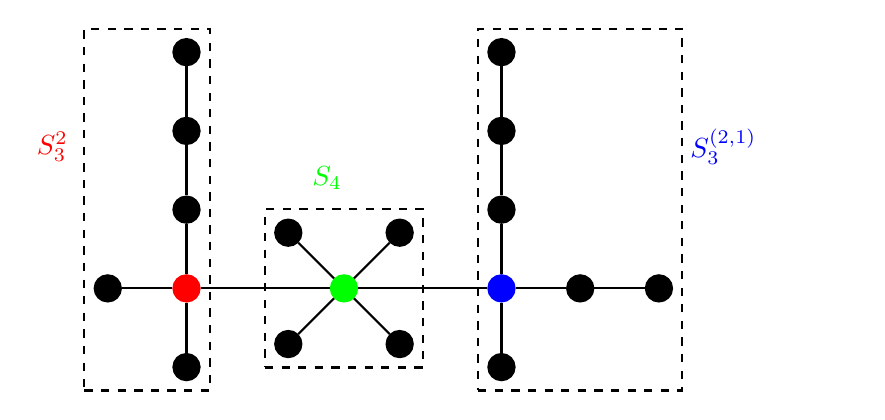
\begin{tikzpicture}[baseline=(current bounding box.north),-,auto,node distance=1cm,
                    thick,main node/.style={circle,draw,fill=black,font=\sffamily\bfseries}]
%first section
  \node[main node,color=red] (1) {};
  \node[main node] (2) [above of=1] {};
  \node[main node] (3) [above of=2] {};
  \node[main node] (4) [above of=3] {};
  \node[main node] (5) [below of=1] {};
  \node[main node] (6) [left of=1] {};
%second section  
  \node[main node,color=green] (7) [shift={(2cm,0cm)}] at (1) {};
  \node[main node] (8) [above left of=7] {};
  \node[main node] (9) [above right of=7] {};
  \node[main node] (10) [below left of=7] {};
  \node[main node] (11) [below right of=7] {};
%third section  
  \node[main node,color=blue] (12) [shift={(2cm,0cm)}] at (7) {};
  \node[main node] (13) [above of=12] {};
  \node[main node] (14) [above of=13] {};
  \node[main node] (15) [above of=14] {};
  \node[main node] (16) [right of=12] {};
  \node[main node] (17) [right of=16] {};
  \node[main node] (18) [below of=12] {};
  

  

  \path[every node/.style={font=\sffamily}]
  (1) edge (2)
  (2) edge (3)
  (3) edge (4)
  (1) edge (5)
  (1) edge (6)
  
  (1) edge (7)
  (7) edge (8)
  (7) edge (9)
  (7) edge (10)
  (7) edge (11)
  
  (7) edge (12)
  (12) edge (13)
  (13) edge (14)
  (14) edge (15)
  (12) edge (16)
  (16) edge (17)
  (12) edge (18);
  
  \node (Box1) [draw,dashed,rectangle,fit=(4) (5) (6)] {};
  \node [shift={(-0.4cm,0.8cm)},text width=2cm,color=red] at (Box1) {$S_{3}^{2}$};  
  
  \node (Box2) [draw,dashed,rectangle,fit=(8) (11)] {};
  \node [shift={(0.6cm,1.4cm)},text width=2cm,color=green] at (Box2) {$S_{4}$};
  
  \node (Box3) [draw,dashed,rectangle,fit=(15) (17) (18)] {};
  \node [shift={(2.4cm,0.8cm)},text width=2cm,color=blue] at (Box3) {$S_{3}^{(2,1)}$};

   
\end{tikzpicture}

\end{center}

\end{frame}

\begin{frame}{\resizebox{\dimexpr\paperwidth - 3ex}{!}{Example of Theorem Applied to joined extended star graphs}}
As the values of the star graphs joined together are
\begin{itemize}
\item $V(S_{3}^{2})=\frac{m}{10}$ when $m \geq 6$
\item $V(S_{4})=\frac{m}{8}$ when $m \geq 2$
\item $V(S_{3}^{(2,1)})=\frac{m}{12}$ when $m \geq 6$
\end{itemize}
To join these together by the centres we will require that $6 \leq m \leq 8$ (hence none of the individual extended star graphs values are invalid), then we will get a value of $V=\frac{m}{30}$. This is achieved by the attacker attacking as they would on individual graphs and the patroller playing on these 3 graphs with the probabilities $\frac{10}{30},\frac{8}{30},\frac{12}{30}$ respectively.
\end{frame}

\begin{frame}{Problem with joining}
The problem with this type of joining is the fact of requiring $m \leq 2\left(n_{i}+\sum\limits_{j} (V_{j})_{i}\right)$.

This is required as otherwise, time is wasted by the patroller when they can be certain that the attacker is not there. Consider the fact that they are $m$ away from the end and they then check all points, then they can move away from the graph and possibly catch some other attacks on other joined extended star graphs.
\end{frame}

\begin{frame}{Example of problem}
Consider $Q$, made by joining the centres of two copies $S_{2}$. Then we know by the theorem that $V(Q)=\frac{m}{8}$ when $2 \leq m \leq 4$, but when $m=5$ say then the problem is that we know that playing in either of them with probability $\frac{1}{2}$ is no longer the best decision. It might be best to count from the starting star's centre
\end{frame}

\end{document}